\documentclass[10pt]{article}
\usepackage[a4paper,margin=1.9cm]{geometry}
\usepackage{amsmath,amssymb}
\usepackage{graphicx}
\graphicspath{{../}{./}}
\usepackage{float}
\usepackage[dvipsnames]{xcolor}
\usepackage{enumitem}
\usepackage{titlesec}
\usepackage[hidelinks]{hyperref}

% --- compact layout ---
\setlist[itemize]{leftmargin=1.35em,itemsep=1pt,topsep=2pt,parsep=0pt}
\setlength{\parindent}{0pt}
\setlength{\parskip}{3pt}
\titlespacing*{\section}{0pt}{6pt}{3pt}
\titlespacing*{\subsection}{0pt}{4pt}{2pt}
\titleformat{\section}{\normalfont\large\bfseries\color{RoyalBlue}}{\thesection.}{0.5em}{}
\titleformat{\subsection}{\normalfont\bfseries}{}{0em}{}

\newcommand{\code}[1]{\texttt{\small #1}}
\newcommand{\file}[1]{\textcolor{RoyalBlue}{\texttt{\small #1}}}

% \docheader{title}{subtitle}
\newcommand{\docheader}[2]{%
  \begin{center}
    {\LARGE\bfseries #1}\\[2pt]
    {\small #2}
  \end{center}
  \vspace{-4pt}\hrule\vspace{6pt}
}

\begin{document}

\docheader{Adora PINN --- Step 7 debug: the stripe artifact}%
{As-built notes \quad$\cdot$\quad Ivan Milic \quad$\cdot$\quad 2026-09-20 \quad$\cdot$\quad debugging the inversion}

The step-7 inversion fits Stokes $I$ well but the recovered maps show stripes. Investigating the saved
field \file{/dat/milic/adora\_pinn\_develop/inverted\_field.npz} and small controlled tests (the step-7
notebook itself was left untouched).

\subsection*{1. The artifact}
The saved field has \code{n\_freq=64}, $\sigma\approx(2.2,\,2.0,\,5.2)$ (the original bandwidth --- the
later \code{(8,8,8)} default has not been re-pretrained in). Its recovered maps at $z'{=}0$: $T$ tracks the
granulation; \textbf{$v_z$ shows diagonal banding}; $B_z$ is smooth with a few real concentrations but a
faint banded background; \textbf{$v_\mathrm{turb}$ is sparse junk} (essentially unconstrained). A 2-D FFT
of the maps shows all power --- and the encoding's frequencies $B_{xy}$ --- confined to
$|k|\lesssim8$\,cyc/FOV, i.e.\ the field \emph{cannot} represent finer horizontal structure.

\begin{center}
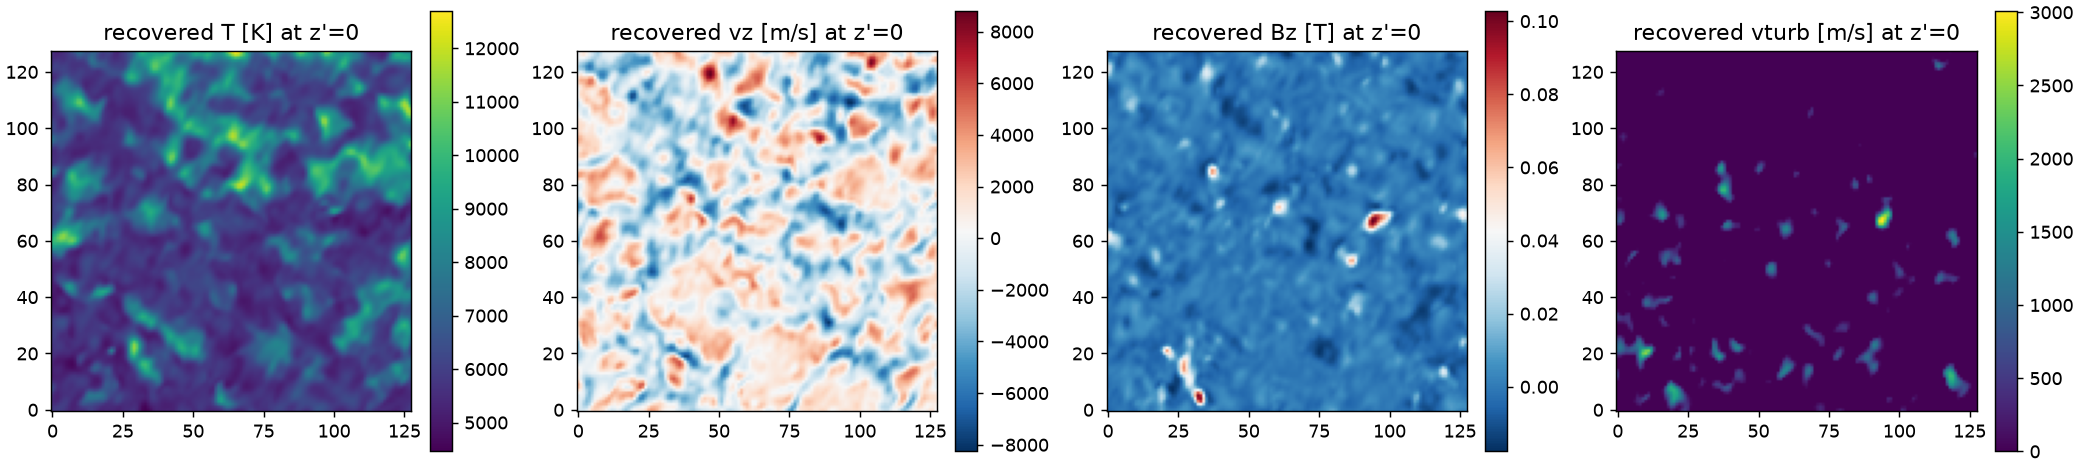
\includegraphics[width=0.99\linewidth]{fig_debug_maps.png}
\end{center}

\subsection*{2. Root cause (controlled test)}
The stripes are the random Fourier modes \textbf{showing through wherever the data under-constrains the
field} (weak channels, and the stochastic per-step pixel sampling). Fitting a fresh 2-D Fourier-MLP to only
\textbf{8\% of the observed-continuum pixels} (the inversion's sparse regime) makes the mechanism explicit:

\begin{center}
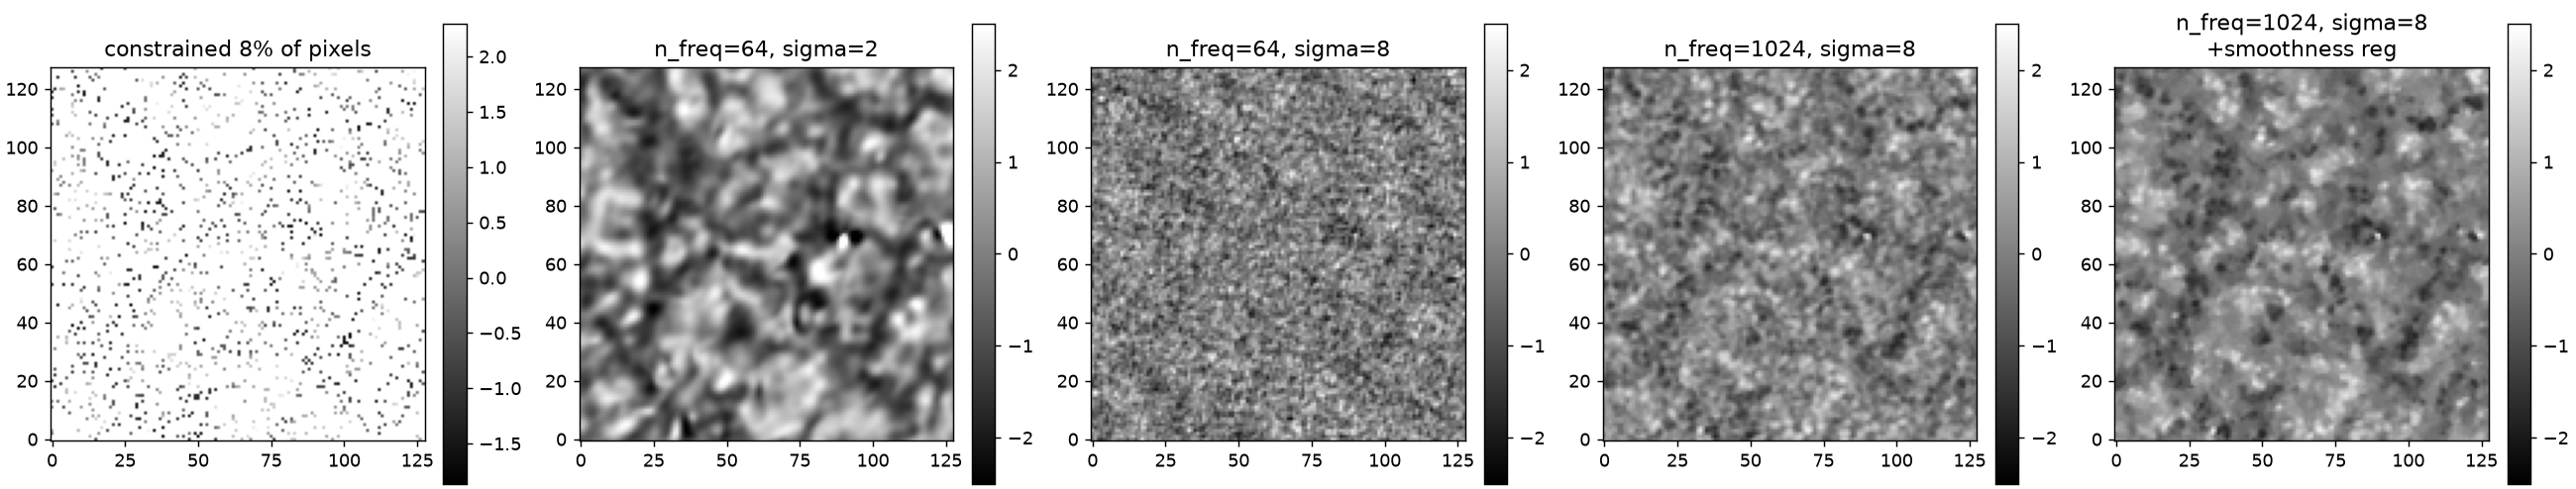
\includegraphics[width=0.99\linewidth]{fig_debug_sparse.png}
\end{center}

\begin{itemize}
  \item $\sigma{=}2$: smooth interpolation but blurry (few low-frequency modes $\to$ the gentle large-scale
        banding seen in $v_z$).
  \item $\sigma{=}8$: \textbf{fine high-frequency ringing} between the constrained points --- \emph{worse}.
        So simply raising $\sigma$ to $8$ would amplify the stripes.
  \item $\sigma{=}8$, \code{n\_freq=1024}: still rings --- \textbf{more features alone does not fix it}.
  \item $\sigma{=}8$ + a \textbf{gradient (smoothness) penalty}: clean \emph{and} high-resolution --- the cure.
\end{itemize}
(A full-batch fit, where every pixel is constrained, hides this: there $\sigma{=}2$ merely under-resolves,
$\sigma{=}8$ is sharp. The stripes are purely an under-constrained-region effect.)

\subsection*{3. Recommendations}
\begin{itemize}
  \item \textbf{Add a spatial-smoothness regularizer} (gradient/TV penalty on the maps, at random points) ---
        the most effective fix; it lets you use a high $\sigma$ for resolution without ringing.
  \item \textbf{Match $\sigma$ to the constraint density}: raising it to $(8,8,8)$ \emph{without} smoothness
        regularization will make the stripes worse, not better.
  \item \textbf{Denser fit sampling} (larger \code{m\_fit}, or occasional full-map steps) --- fewer
        under-constrained pixels per step.
  \item \textbf{Weakly-constrained channels} ($v_\mathrm{turb}$, transverse $B$) should be regularized hard
        or frozen --- they are currently free to absorb stripe junk.
\end{itemize}
Next concrete step (when you want it): add a smoothness term to \file{losses.py} and expose its weight in
\code{run\_inversion}; keep $\sigma$ moderate and re-pretrain the warm start at the chosen bandwidth.

\end{document}
